\chapter{Competizioni CTF A/D}

Le competzioni CTF di tipo attacco/difesa sono una tipologia di competizioni CTF in cui i partecipanti devono difendere i propri servizi
e attaccare i servizi degli avversari, in un contesto di gara estremamente dinamico e competitivo. 
In queste competizione prendono parte diversi team, ai quali viene associato una macchina (solitamente unix-like) con un insieme di servizi,
i quali hanno delle vulnerabilità.\footcite{\url{https://faustctf.net/information/attackdefense-for-beginners/}}{faustctf_attackdefense_for_beginners}
I servizi sono accessibili tramite la rete di gara, e sono replicati in tutte le macchine.

\section{Descrizione dell'infrastruttura}

\subsection{Il Gameserver e i Checker}

Al centro di tutta la competizione c'è il \texttt{gameserver}, servizio che prende in gestione la competizione
calcolando i punteggi e offrendo diversi servizi descritti in questo capitolo essenziali per il suo svolgimento.
La competizione stessa è strutturata in \texttt{tick} (o \texttt{round}),
ovvero intervalli di tempo in cui ciclicamente il gameserver assegna punti ai team in base alle azioni compiute dagli stessi
e monitora i servizi tramite i \texttt{checker} (descritti in seguito).
Questo tempo può variare da competizione a competizione. I \texttt{checker} sono dei bot che si occupano di verificare lo stato della gara eseguendo diverse azioni:
\begin{itemize}
    \setlength{\itemsep}{5pt}
    \setlength{\parskip}{5pt}
    \item Si occupano di verificare se il servizio è funzionante e raggiungibile, andando a connettersi, ed eseguendo azioni
    di normale utilizzo, verificandone anche l'integrita.
    \item Altri si occupano di utilizzare il servizio per memorizzare una \texttt{flag} (solitamente una stringa generata randomicamente) al suo interno,
    avente un formato ben noto fornito dagli organizzatori ed inserita in modo tale da essere non essere normalmente accessibile secondo le logiche del servizio stesso.
    \item Altri ancora si occupano di verificare che le flag dei tick precedenti siano ancora raggiungibili tramite un normale accesso autorizzato e che
    quindi non siano state modificate o rimosse dal team possessore di quella macchina.
\end{itemize}

In generale, rimuovere le vecchie flag, avere il servizio non raggiungibile e l'impossibilità di inserire nuove flag sono azioni che vanno ad invalidare la normale
attività del servizio, e il gameserver lo considererà totalmente o parzialmente inaccessibile o manomesso (dipendentemnte dalle scelte degli organizzatori).\\

Si evidenza come i checker non sfruttino mai le vulnerabilità dei servizi, ma si limitino all'utilizzo corretto degli stessi.

\subsection{I servizi, le flag e i flag store}

Ogni flag viene generata e inserita nel servizio dei vari team ad ogni tick (ogni team avrà una flag differente dagli altri), ed ha usualmente una durata massima di valenza (ad esempio 5 tick):
in questo intervallo di tempo è ancora possibile consegnare la flag, ed ottenere punti consegnandola al gameserver.\\

Le flag infatti una volta ottenute vanno consegnate al gameserver, che tramite un calcolo che varia in diverse competizioni, assegna punti al team che ha consegnato la flag.\\

Nel seguente esempio si mostra il calcolo per l'assegnazione dei punti per una flag consegnata e valida utilizzato nel progetto CyberChallenge\footcite{\url{https://rules.ad.cyberchallenge.it/}}{cyberchallenge_ad_rules}:

\begin{listing}[H]
    \begin{minted}[
        frame=single,
        framerule=0.8pt,
        fontsize=\footnotesize,
        breaklines
      ]{python}
scale = 15 * sqrt(5) 
norm = ln(ln(5)) / 12 
offense_points[flag] = scale / (1+exp((sqrt(score[attacker][service]) - sqrt(score[victim][service]))*norm))
defense_points[flag] = min(victim_score, offense_points)
\end{minted}
\end{listing}

Il defense point è il punteggio sottratto al team da cui è stata rubata la flag come verrà meglio descritto in seguito.\\

Si da per assodato che consegnare le flag del proprio team non da alcun punteggio, in quanto il gameserver sa già quali sono le flag generate per il proprio team, ne tantomeno 
le flag rubate da dei team 'di prova' (spesso chiamati \texttt{NOP team}) che sono semplicemente macchine non associate a nessun team, che offrono i medesimi servizi
al solo scopo di renderli usufruibili per eseguire dei penetartion testing (non tutte le competizioni prevedono la presenza dei \texttt{NOP team}).\\

Una differenziazione importante da sottolineare riguarda il significato di \texttt{servizio} di cui si è parlato fino ad ora:
si è implicitamente assunto che per ogni servizio ci sia 1 sola flag per tick e che per ogni servizio ci sia 1 sola vulnerabilità.
Questo spesso non è vero, poichè ogni servizio ha usualmente più vulnerabilità, ma non solo, potrebbe avere anche diverse flag per tick a suo interno:
i checker che si occupano di inserire le flag potrebbero inserirne diverse, in diverse parti del servizio.
In caso di servizi con più flag, diremo che quel servizio avrà più \texttt{flag store}.
Ciò detto prima e ciò che verrà detto in seguito è valido per ogni flag store, tuttavia spesso continueremo a parlare comunque di servizi per semplicità.

\subsection{I Flag ID}

Il gameserver potrebbe rilasciare delle informazioni aggiuntive per ogni servizio, come ad esempio un username, che di per se non vanno
ad esporre in modo diretto ad esempio le credenziali per accedere ad una pagina protetta contenete la flag, ma danno un infomazione utile agli attaccanti al fine di poter
individuare più facilmente la flag all'interno del servizio stesso.
Questa informazione aggiuntiva è chiamata \texttt{Flag ID} e viene rilasciata per ogni team, per ogni flag store, e per ogni flag ancora valida nel momento in cui si visita l'API che
le espone pubblicamente per tutti i partecipanti (resa disponibile dal gameserver). Non è possibile manomettere i flag id, in quanto contengono informazioni direttamente rilasciate dagli organizzatori, e che comunque in assenza di
vulnerabilità nei servizi non sono sufficienti al fine di ottenere delle flag.

\subsection{Calcolo del punteggio}

Il calcolo del punteggio associato ad ogni team è composto da diversi punteggi parziali, ogniuno riguardante 1 flag store (che per semplicità chiameremo servizio).
Usualmente infatti ad ogni servizio è associato un punteggio base da cui partire, che poi viene modificato durante la competizione in base a dei sotto punteggi parziali descritti in seguito:
\begin{itemize}
    \setlength{\itemsep}{5pt}
    \setlength{\parskip}{5pt}
    \item Il punteggio di \texttt{SLA} (Service Level Agreement) riguarda la disponibilità del servizio, e che viene calcolato in base al tempo in cui il servizio è stato up o down.
    Questo è il punteggio che solitamente ha più peso rispetto agli altri, e spesso viene applicato come percentuale sul totale del punteggio del servizio. Questo accade al fine di
    rendere totalmente insignificante l'idea di spegnere i servizi con lo scopo di evitare di subire attacchi, penalizzando fortemente questa pratica.
    La normale attività del servizio (seppur vulnerabile) pertanto diventa di vitale importanza nella competizione.
    \item Il punteggio di \texttt{attacco} è calcolato in base alle submission di flag eseguite dal team. Il punteggio per ogni flag può variare in base alla difficoltà dell'attacco,
    alle condizioni generali di gara e alla velocità con cui si è riusciti ad attaccare quel servizio (come visto precendetemente).
    \item Il punteggio di \texttt{difesa} (solitamente negativo poichè considera quanto "male" ci si sia difesi) è calcolato in base alle consegne
    delle proprie flag eseguite dai team avversari. Accade spesso che questo punteggio vada a controbilanciare il punteggio di attacco sullo stesso servizio, se non a farlo decadere, andando anche a
    ribasso del punteggio base assegnato, ed è variabile in base agli stessi criteri del punteggio di attacco. Per questo motivo diventa necessario eseguire
    fix o patch sui propri servizi, impedendo l'arrivo nuovi attacchi (ma comunque mantenendo il servizio in piena attività),
    e mantenendo anche i vecchi dati (e quindi anche le vecchie flag, non compromettendo per quanto possibile il punteggio di SLA).
\end{itemize}

\texttt{NOTA:} Comunemente esiste un checker differente per ogni servizio.

\vspace{\fill}
\newpage

Di seguito si riporta come viene calcolato il punteggio nelle competizioni nazionali attack defence di Cyberchallenge\footcite{\url{https://rules.ad.cyberchallenge.it/}}{cyberchallenge_ad_rules}:

\begin{listing}[H]
    \begin{minted}[
        frame=single,
        framerule=0.8pt,
        fontsize=\footnotesize,
        breaklines
      ]{python}
# -- Total score for each service (or better said, flag store)

# Service base points 
score[team][service] = 5000 
            
# Sum offensive points 
for flag in stolen_flags[team][service]:
    score[team][service] += offense_points[flag] 
    
# Substract defensive points 
for flag in lost_flags[team][service]: 
    score[team][service] -= defense_points[flag]

# -- Final team score

total_score[team] = 0 
        
for service in services: 
    # Compute SLA of the service
    sla[team][service] = ticks_up[team][service] / ticks[team][service] 
    # Limit scores to 0
    score[team][service] = max(0, score[team][service]) 
    # Add service score
    total_score[team] += score[team][service] * sla[team][service]

\end{minted}
\end{listing}

\newpage

\subsection{Rete di gara}

Di seguito si prende in considerazione la rete di gara in utilizzo per le competizioni
nazionali di Cyberchallenge\footcite{\url{https://rules.ad.cyberchallenge.it/}}{cyberchallenge_ad_rules}:

\begin{figure}[H]
    \centering
    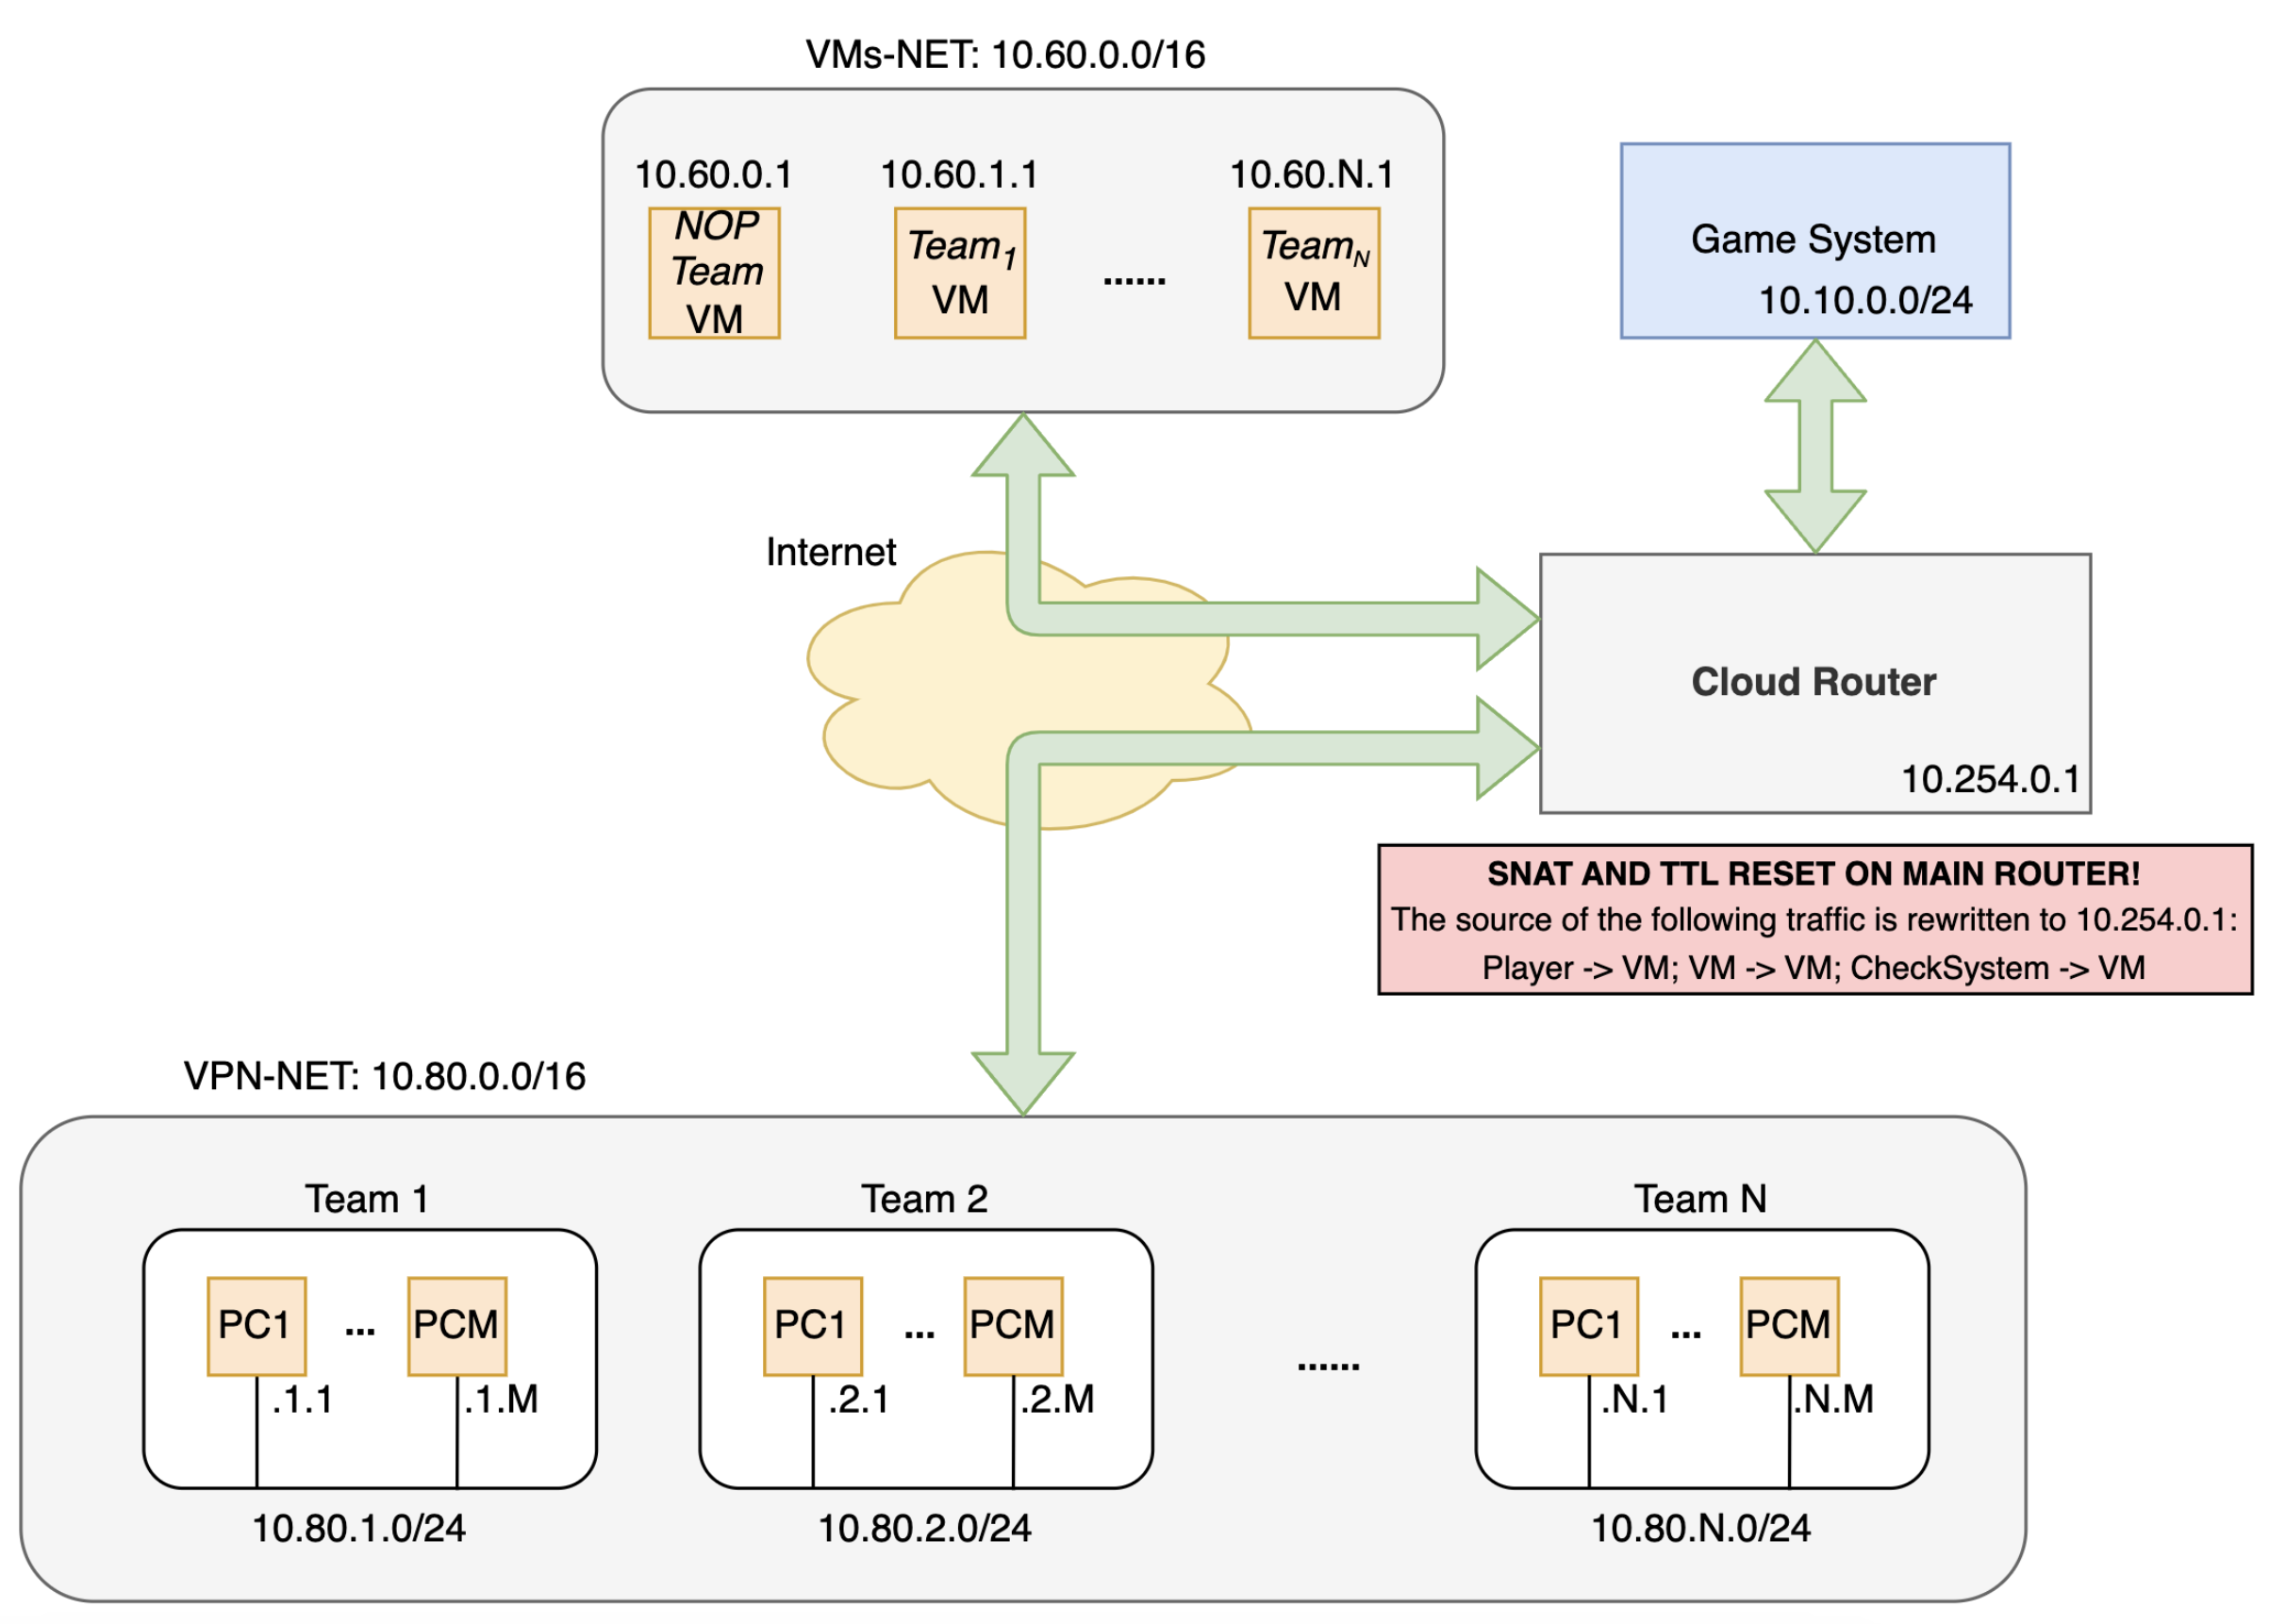
\includegraphics[width=0.8\textwidth]{images/chapter1/ccit_network.png}
    \caption{Modello della rete di gara di Cyberchallenge}
    \label{fig:ccit_network}
\end{figure}

Come si può vedere nella figura \ref{fig:ccit_network} la rete di gara è composta da diversi elementi:
\begin{itemize}
    \setlength{\itemsep}{5pt}
    \setlength{\parskip}{5pt}
    \item La rete dedicata agli organizzatori, dove abbiamo il gameserver ed eventuali altri host al servizio degli organizzatori o del gameserver stesso.
    \item La sottorete delle macchine dei team, dove ogni team ha accesso ssh alla sua macchina con i servizi vulnerabili.
    \item Una sottorete (spesso realizzata tramite VPN) per ogni team dove sono connessi i laptop dei partecipanti dalla quale possono accedere alla rete di gara.
\end{itemize}

Al centro di tutto ciò abbiamo il cloud router, che si occupa di gestire il traffico in base alle regole impostate dagli organizzatori e allo stato della competizione, ma
soprattutto che si occupa di \texttt{anonimizzare il traffico} manipolandolo tramite diverse tecniche tra le quali la principale è il \texttt{NAT} (Network Address Translation).
Tramite il \texttt{NAT} infatti si nascondono gli indirizzi IP delle macchine e dei componenti del team, mascherando nelle richieste l'ip con quello (o quelli) del router.
Quest'ultimo elemento è fondamentale poichè altrimenti sarebbe semplice diversificare le connessioni dei checker e degli attaccanti, e si andrebbe a perdere l'obiettivo che ha
la competizione stessa, ovvero individuare, sfruttare e difendersi dalle vulnerabilità.

Inoltre le reti dei componenti del team sono isolate per tutta la competizione, e questo al fine di evitare possibili attacchi agli host dei partecipanti,
considerata generalmente una pratica scorretta e non conforme alla gara, che potrebbe portare alla squalifica del team attaccante.

\section{Svolgimento della competizione}

Una competizione A/D inizia dal momento in cui viene dato accesso alle macchine e alla rete di gara. Usualmente in questa fase c'è un periodo di tempo
in cui la rete di gara è chiusa: i team hanno accesso unicamente alle loro macchine e ne le macchine stesse ne i componenti del team possono comunicare con le macchine degli avversari.\\
In questo momento è possibile però analizzare i servizi, avviare tutti i tool necessari all'avvio degli attacchi, all'analisi della rete, e alla difesa del server (che analizzeremo nel prossimo paragrafo).
Finito questo periodo di tempo, la rete di gara viene aperta, e la competizione inizia ufficialmente.\\
Da questo momento il gameserver inizia a scandire i tick, i checker iniziano ad utilizzare i servizi e ad inserire le prime flag, pubblicando i primi flag id.
I team iniziano a lavorare, tentando di difendersi dai primi attacchi, e a loro volta di attaccare rubando le flag degli avversari, cercando sempre di mantenere i loro servizi attivo e funzionante.
Ogni tick il gameserver assegna i punti, e i team possono vedere il proprio punteggio e quello degli avversari, comprendendo le prossime azioni da compiere per massimizzare il punteggio.
Inoltre viene segnalato pubblicamente quali servizi di quale team non sono funzionanti, e perchè sono considerati down (cioè la motivazione per cui i checker hanno segnalato un mal funzionamento).
La competizione termina ad un determinato orario di fine, dove la rete di gara viene chiusa, e il gameserver interrompe l'azione dei checker, e non accetta nuove submission di flag.\\

\texttt{NOTA:} tutto ciò descritto in questo paragrafo è possibile simularlo e sperimentarlo con un mio progetto chiamato \texttt{Oasis}\footcite{\url{https://github.com/domysh/Oasis}}{oasis_gh},
fork del progetto originale dei TheRomanXpl0it\footcite{\url{https://theromanxpl0.it/about.html}}{theromanxploit} con cui è possibile simulare ma anche 
svolgere una competizione A/D di medio-piccole dimensioni in un ambiente simulato unicamente con l'utilizzo di container podman ispirato a CyberChallenge.

\section{Tool utili}

Data l'elevata complessità nello svolgimento di una competizione A/D, spesso diventa necessario l'utilizzo di diversi tool che permettano di automatizzare
diverse operazioni necessarie nella gara. Ogni team può sviluppare e utilizare tool che facilitano (o per fino che automizzino) l'attacco e la difesa dei servizi.\\
In generale sono frequenti nel loro utilizzo le seguenti categorie di tool:

\begin{itemize}
    \setlength{\itemsep}{5pt}
    \setlength{\parskip}{5pt}
    \item \texttt{Traffic Analyzer} che permettono di analizzare il traffico sulla macchina, in modo da riconoscere e visonare il traffico dei checker e degli attaccanti.
    Analizzare il traffico diventa cruciale dal momento in cui un nuovo attacco è attivo sulla rete, poichè permette al team di analizzare l'attacco, riconoscere la vulnerabilità
    sfruttata dai team avversari, e intraprendere azioni quanto più immediate per la difesa e l'attacco con l'utilizzo della stessa falla. Normalmente per analizzare il traffico è
    possibile usare tool quali \texttt{Wireshark}\footcite{\url{https://www.wireshark.org/}}{wireshark} o \texttt{Suricata}\footcite{\url{https://suricata.io/}}{suricata} (anche se non propriamente un network analyzer).
    Solitamente però non si utilizzano tool simili dato il loro poco pratico utilizzo in ambito CTF A/D dove il traffico da analizzare è elevato e continuo.
    Esistono tool scritti appositamente per queste competizioni che permettono di analizzare il traffico in modo più efficiente e veloce, ma anche di riprodurre velocemente
    le stesse sequenze di attacco, come ad esempio \texttt{Caronte}\footcite{\url{https://github.com/eciavatta/caronte}}{caronte} o
    \texttt{Tulip}\footcite{\url{https://github.com/OpenAttackDefenseTools/tulip}}{tulip} (che utilizza internamente suricata).
    \item \texttt{Attacker \& Submitter} che coordinano gli attacchi, assistono alla scrittura degli exploit, ne monitorano l'esecuzione, la schedulano e la paralellizzano.
    Questi tool sono fondamentali per l'attacco e hanno lo scopo di far concentrare l'attaccate sulla scrittura del singolo attacco, e non sulla gestione dell'esecuzione dell'
    attacco stesso. Inoltre spesso viene offerta la possibilità di monitorare gli attacchi al fine di osservare facilmente problemi nell'esecuzione e 
    quanti e quali team stanno iniziando a difendere il servizio. Usualmente (ma non sempre) questi tool eseguono anche la parte di submission delle flag al gameserver, che
    avviene in modo centralizzato per tutte le flag di tutti i servizi, poichè spesso diventa così più semplice coordinare la consegna delle flag in base alle regole che gli organizzatori impongono sul numero di submission per evitare 
    attacchi di tipo \texttt{bruteforce} o \texttt{DoS} all'infrastruttura. Tool di questo genere sono ad esempio \texttt{DestructiveFarm}\footcite{\url{https://github.com/DestructiveVoice/DestructiveFarm}}{destructivefarm}, che
    tuttavia ha diversi punti deboli e non ha una serie di funzionalità sull'analisi dell'andamento degli attacchi, motivo per il quale ho sviluppato un nuovo tool chiamato
    \texttt{ExploitFarm}\footcite{\url{https://github.com/Pwnzer0tt1/exploitfarm}}{exploitfarm} che permette di coordinare gli attacchi, di monitorarli, e di schedularli in modo più efficiente e semplice.
    \item \texttt{Proxy} che permettono di filtrare il traffico in modo da riconoscere e bloccare gli attacchi. Questi tool possono essere molto utili
    nella difesa, e permettono di riconoscere e bloccare gli attacchi evitando la modifica dei servizi stessi, causa comune di down del servizio.
    Questo modo di progettere i servizi è spesso incompleto e bypassabile, ma se ben progettato e ben utilizzato può essere un'ottima soluzione temporanea, se non
    una soluzione completa in alcune casistiche per la difesa. Spesso però la soluzione più efficace rimane quella di correggere la vulnerabilità.
    Tool di questo genere sono ad esempio \texttt{CTF Proxy}\footcite{\url{https://github.com/ByteLeMani/ctf_proxy}}{ctf_proxy} o il tool di cui tratta questa tesi \texttt{Firegex}\footcite{\url{https://github.com/Pwnzer0tt1/firegex}}{firegex_gh}.
\end{itemize}

